\section{Evaluation}
\label{gen:sec:expr}

The evaluation aims to answer the following questions:
\begin{enumerate}[leftmargin=0.5cm]
       \item  How does \genrewrite compare to a straighforward application of the out-of-the-box LLM? In other words, do our   NLR2s and counterexample-based correction algorithm considerably boost the LLM's performance? (\S\ref{gen:sec:expr:llmbaseline})

\item How does \genrewrite compare to state-of-the-art rule-based query rewriting approaches? Specifically, which approach can optimize more queries and which approach yields more speedup for the rewritten queries? (\S\ref{gen:sec:expr:traditionalbaseline})

\item  How much does each of \genrewrite's design contribute to its overall success (ablation study)?   (\S\ref{gen:sec:expr:ablation})

\item  What is the time and monetary cost of \genrewrite?  (\S\ref{gen:sec:expr:llmcost})

% \item How does the choice of the LLM with various capabilities influence the effectiveness of \genrewrite's rewrites? (\S\ref{gen:sec:expr:llmchoice})
\end{enumerate}

\subsection{Experimental Setup}
\label{gen:sec:expr:setup}

\genhead{Testbed} Our experiments are all conducted on Google Cloud Engine Machine n2-highmem-2 instances, with with 16GB RAM and 2 vCPUs. We use PostgreSQL 14.17. To evaluate query latency accurately, we execute each query 3 times and take their average as the final latency value. \revthree{We do not create any indexes. Instead, we run \texttt{VACUUM ANALYZE} on all tables before benchmarking, which collects statistics for cost-based plan selection.}


\cut{Before each run, we restart the PostgreSQL service and clear the database cache.} \cut{revise later, we have an off-shelf SQL verifier that works for some TPC-DS queries and most JOB queries Additionally, we use an off-the-shelf tester from~\cite{dong2023slabcity} to check query equivalence followed by manual inspection.}



% we generate a carefully designed dataset of small size to verify the correctness of our query rewrites.


\genhead{Choice of LLM} We designate OPENAI o3-mini as the default LLM, due to its cost efficiency and robust reasoning capabilities. We also assess \genrewrite's generalizability across other LLMs with varying capabilities, such as GPT-4o and GPT-4-mini.


\genhead{Workloads} \revtwo{Our experiments include two widely used analytical benchmarks, TPC-DS~\cite{tpcds} and the Join Order Benchmark (JOB)~\cite{leis2015good}, as well as additional query sets generated by SQLStorm~\cite{schmidt2025sqlstorm} over the same TPC-DS and JOB schemas. SQLStorm uses LLMs to synthesize thousands of executable, high-complexity SQL queries and then filters them using actual database feedback. These SQLStorm queries were released in June 2025—after the pretraining cutoff of the LLM we use (October 2023)—and thus were not available during pretraining, allowing us to assess how well \genrewrite generalizes to previously unseen queries on familiar schemas.}


% We evaluate \genrewrite on multiple workloads to test its robustness across schema and query complexity. 




% To verify the effectiveness of \genrewrite across different scenarios, we conduct experiments on two workloads: TPC-DS and JOB. Besides these two standard benchmarks, we also include queries generated by SQLStorm under the same public schema, which is unknown to the LLMs, so that we can test how our methods performs

\begin{enumerate}[leftmargin=0.5cm]


\item \textbf{TPC-DS.}
TPC-DS is an industry-standard decision support benchmark. While it does not perfectly capture the recurring, user-specific workloads seen in production, it remains a strong proxy for realistic analytical queries and is widely used to compare query optimization techniques. We generated a 10\,GB TPC-DS instance and used all 99 benchmark queries.

\item \textbf{Join Order Benchmark (JOB).}
JOB is a canonical benchmark derived from the IMDB dataset and is heavily used to study join ordering and cost-based optimization. Its queries span diverse levels of complexity and involve multi-way joins, making it a good stress test for optimizer behavior.

\item \textbf{\revtwo{TPC-DS (SQLStorm).}}
\revtwo{SQLStorm generated tens of thousands of query variants over the TPC-DS schema. Running LLM-based methods on all of them would be prohibitively expensive due to LLM inference cost. We therefore select the 100 slowest SQLStorm-generated queries as measured by runtime under \texttt{olapbench}~\cite{OLAPBench}. According to SQLStorm's own analysis, these queries fall in the medium-to-high complexity range.}

\item \textbf{\revtwo{JOB (SQLStorm).}}
\revtwo{We apply the same selection criterion for JOB: We select the 50 slowest queries by runtime under \texttt{olapbench}. As with the TPC-DS (SQLStorm) set, these queries are classified as medium to high complexity.}


\end{enumerate}

\genhead{Baselines} We compare \genrewrite against two LLM-based approaches and three state-of-the-art rule-based query rewriting methods, two of which, \textsc{LLM-R\textsuperscript{2}} and \rbot, incorporate LLMs:
\begin{itemize}[leftmargin=0.5cm]
    \item \textbf{\baseline} employs a basic prompting technique illustrated in Figure~\ref{gen:fig:basic_prompt} to generate candidate queries without any correction mechanism. 
        This baseline represents the straightforward application of out-of-the-box LLM.

        \item \revone{\textbf{LITHE}~\cite{llm-rw2} is an LLM-based method that constructs a database-sensitive prompt by selecting the most appropriate  rule for the input query from a fixed set of six handcrafted rules. These rules target redundancy elimination and selectivity improvement.}
        
  

    \item \genjie{\textbf{LLM-R\textsuperscript{2}} (VLDB 2025~\cite{li2024llm})  is an LLM-enhanced query rewrite system that can automatically select effective rules from a given set of rewrite rules to rewrite an input SQL query by leveraging a high-quality demonstration pool.}

    \item \textbf{R-Bot} (VLDB 2025~\cite{sun2024r}) is a query rewrite system that retrieves the most relevant rewrite evidences and employs an LLM-driven, step-by-step method to iteratively select and arrange rewrite rules based on retrieved evidence.

      \item \textbf{LearnedRewrite} (or \textbf{LR}, VLDB 2022~\cite{LR}) is a state-of-the-art rule-based query rewriter~\cite{LR} which uses Monte Carlo Tree Search to guide the rule-based rewriting process. LR uses rewrite rules from Calcite~\cite{begoli2018apache}, which is the most popular library for query rewriting rules.


% \genhead{\revone{Comparison with QUITE~\cite{song2025quite}}} \revone{QUITE\cite{song2025quite} is also an LLM-based method for rewriting SQL queries beyond rules. However, the authors have not released code or several critical components (including the curated knowledge base and the LLM-based SQL corrector). Without access to these pieces, we cannot responsibly and confidently perform a direct experimental comparison. We therefore focus on high-level differences. QUITE models the query rewrite process as a Markov Decision Process and at each timestep it chooses a refinement action (e.g., join reordering, predicate pushdown) by matching the query against a curated knowledge base constructed from database documentation and Stack Overflow\cite{stackoverflow}. This constrains the search space to optimizations that are explicitly documented. By contrast, \genrewrite is not limited to a predefined action library. It can  apply optimization strategies that are implicitly encoded in the LLM  and accumulate novel patterns as NLR2s over time .}







% Since the authors have not published the code and some key components, e.g., curated knowledge base and the prompts for LLM-based SQL corrector, we cannot responsibly and confidently compare with their method. So we compare the high-level differences instead. It models the query rewrite process as a Markov Decision Process and at each timestep the agent chooses a refinement action (e.g., join reordering, predicate pushdown) based on the match with curated knowledge base, which is constructed from official database documentation and Stack Overflow~\cite{stackoverflow}. The issue is that this limits LLM's expressiveness and capabilities to apply patterns not explicitly listed in above resources to the query to achieve great speedups.





    

\end{itemize}

Note that while both \textsc{LLM-R\textsuperscript{2}} and \rbot utilize LLMs to enhance rule selection and sequencing, they do not explore beyond the space defined by the existing rule set. Therefore, we still classify them as rule-based approaches. We excluded ~\cite{wetune} from our experiments as it was not able to produce valid rewrites for any TPC-DS queries.

\genhead{Setup} \genjie{Rule-based query rewriting methods produce the same rewrite for an input query across multiple runs. In contrast, due to the statistical nature of LLMs,} additional LLM runs increase the likelihood of uncovering new rewrite possibilities and thereby improving performance.  To ensure a fair comparison across approaches, we fix the number of iterations for each LLM-based method to four, generating four rewrite candidates per query. \baseline  uses the basic prompt (see Figure~\ref{gen:fig:basic_prompt}) in all four iterations, without any correction or contextual enhancement.  \genrewrite also uses the basic prompt in the first iteration, \revone{as the NLR2 Repository is initially empty and we do not use pre-seeded or external rules}. In subsequent iterations, it selectively incorporates relevant and beneficial NLR2s retrieved from the repository, if such rules are available, to guide the rewriting process more effectively. \revone{The semantic- and syntax-correction loops are each capped at 3 iterations. If, after these caps, a candidate still fails semantic correction or remains unparsable by the DBMS, we discard it and retain the original input $q$.} A method is considered successful on the given query $q$ if any of these four candidates is both equivalent to the original query and faster. If any method, rule-based or LLM-based, fails to produce an equivalent rewrite for the given query, we assign a speedup ratio of 1, indicating that the original query is used as a fallback.

% we generate four rewrites for each LLM-based method: both Baseline LLM and \genrewrite share the first two candidate rewrites generated using the basic prompt (see Figure~\ref{gen:fig:basic_prompt}), while the remaining two candidates differ—\genrewrite incorporates the NLR2 with the highest estimated benefit as the hint, whereas Baseline LLM continues using the basic prompt. 

% A method is considered successful if any of these four candidates is both equivalent to the original query and faster. Additionally, if any method, rule-based or LLM-based, fails to produce an equivalent rewrite for a particular query, we deem the speedup ratio for that query as 1, indicating a fallback to the original query.


    % \item
    % \cut{ \textbf{Fusion} Computation Reuse via Fusion~\cite{bruno2022computation} is a technique for rewriting complex SQL queries in Amazon Athena. It focuses on minimizing computational redundancy by identifying and merging repeated operations, including instances where the common expressions are not exactly the same.}

% Both techniques had been evaluated on TPC-H or Leetcode~\cite{??} queries, which are much simpler than TPC-DS.












\begin{table}[tbp]
% \small
\footnotesize
\centering
\setlength{\tabcolsep}{5pt}
\def\arraystretch{1.1}
\vspace{-5pt}

\begin{subtable}[t]{0.48\textwidth}
\centering
\begin{tabular}{  c | r r r | r r r }
\toprule
& \multicolumn{3}{c|}{TPC-DS} 
& \multicolumn{3}{c}{JOB} \\
speedup & >2x & >10x & >50x & >1.2x & >2x & >10x \\
\midrule
\genrewrite     & \makecell{25\\(25.3\%)} & \makecell{9\\(9.1\%)}  & \makecell{6\\(6.1\%)}  & \makecell{20\\(17.7\%)} & \makecell{8\\(7.1\%)}  & \makecell{3\\(2.7\%)} \\
\baseline & \makecell{18\\(18.2\%)} & \makecell{6\\(6.1\%)}  & \makecell{5\\(5.1\%)}  & \makecell{19\\(16.9\%)} & \makecell{7\\(6.2\%)}  & \makecell{3\\(2.7\%)} \\
\revone{\lithe} & \makecell{16\\(16.2\%)}    & \makecell{6\\(6.1\%)}  & \makecell{4\\(4.0\%)}    & \makecell{17\\(15.0\%)}    & \makecell{6\\(5.3\%)}    & \makecell{1\\(0.9\%)} \\
\textsc{LLM-R\textsuperscript{2}} 
          & \makecell{10\\(10.1\%)} & \makecell{6\\(6.1\%)}  & \makecell{5\\(5.1\%)}  & \makecell{9\\(8.0\%)}   & \makecell{2\\(1.8\%)}  & \makecell{1\\(0.9\%)} \\
\rbot     & \makecell{9\\(9.1\%)}   & \makecell{5\\(5.1\%)}  & \makecell{3\\(3.0\%)}  & \makecell{7\\(6.2\%)}   & \makecell{3\\(2.7\%)}  & \makecell{2\\(1.8\%)} \\
\lr       & \makecell{6\\(6.1\%)}   & \makecell{4\\(4.0\%)}  & \makecell{0\\(0\%)}    & \makecell{6\\(5.3\%)}   & \makecell{2\\(1.8\%)}  & \makecell{1\\(0.9\%)} \\
\bottomrule
\end{tabular}
\captionsetup{font=small}
\caption{Original workloads.}
% \inv
\label{gen:tab:speedup_comparison}
\end{subtable}

\hfill

\begin{subtable}[t]{0.48\textwidth}
\centering
\begin{tabular}{  c | r r r | r r r }
\toprule
& \multicolumn{3}{c|}{TPC-DS (SQLStorm)} 
& \multicolumn{3}{c}{JOB (SQLStorm)} \\
speedup & >2x & >10x & >50x & >1.2x & >2x & >10x \\
\midrule
\genrewrite     & \makecell{25\\(25.0\%)} & \makecell{13\\(13.0\%)}  & \makecell{3\\(3.0\%)}  & \makecell{7\\(14.0\%)} & \makecell{6\\(12.0\%)}  & \makecell{1\\(2.0\%)} \\
\baseline & \makecell{12\\(12.0\%)} & \makecell{9\\(9.0\%)}  & \makecell{3\\(3.0\%)}  & \makecell{4\\(8.0\%)} & \makecell{2\\(4.0\%)}  & \makecell{1\\(2.0\%)} \\
\revone{\lithe}    & \makecell{19\\(19\%)}    & \makecell{11\\(11.0\%)}  & \makecell{2\\(2.0\%)}    & \makecell{6\\(12.0\%)}    & \makecell{4\\(8.0\%)}    & \makecell{1\\(2.0\%)} \\
\textsc{LLM-R\textsuperscript{2}} 
          & \makecell{2\\(2.0\%)} & \makecell{1\\(1.0\%)}  & \makecell{0\\(0.0\%)}  & \makecell{2\\(4.0\%)}   & \makecell{2\\(4.0\%)}  & \makecell{0\\(0.0\%)} \\
\rbot     & \makecell{2\\(2.0\%)}   & \makecell{0\\(0.0\%)}  & \makecell{0\\(0.0\%)}  & \makecell{2\\(4.0\%)}   & \makecell{2\\(4.0\%)}  & \makecell{0\\(0.0\%)} \\
\lr       & \makecell{4\\(4.0\%)}   & \makecell{1\\(1.0\%)}  & \makecell{0\\(0\%)}    & \makecell{3\\(6.0\%)}   & \makecell{1\\(2.0\%)}  & \makecell{0\\(0.0\%)} \\
\bottomrule
\end{tabular}
\captionsetup{font=small}
\caption{\revtwo{SQLStorm-generated workloads.}}
\label{gen:tab:speedup_comparison_sqlstorm}
\end{subtable}



\captionsetup{font=small,name=Table}
\caption{Speedup comparison beyond thresholds between all methods. Upper: original TPC-DS and JOB. Lower: SQLStorm-generated TPC-DS and JOB. We report absolute counts and percentages to reflect the different workload sizes.}
\label{gen:tab:speedup_all}
\vspace{-15pt}
\end{table}


\subsection{Comparison with \revone{LLM-based Methods}}
\label{gen:sec:expr:llmbaseline}


Table~\ref{gen:tab:speedup_all} compares the fraction of queries that each method speeds up beyond several thresholds. Before discussing individual results, we note an important trend: queries in JOB are generally less complex than those in TPC-DS, both in the original benchmarks and in the SQLStorm-generated variants. In the original workload, JOB queries average 278.81 tokens, whereas TPC-DS queries average 441.34 tokens (a 58\% increase). Although JOB queries can involve many joins and are therefore challenging for join ordering, their overall structure is simpler: they contain fewer nested subqueries, window functions, and set operations than TPC-DS. \revtwo{This gap persists in the SQLStorm workloads. Even when SQLStorm generates new queries with medium to high complexities over both schemas, the JOB-derived queries remain constrained by narrower, more normalized tables and by the absence of complex cross-channel or temporal comparisons. This difference in query complexity translates to different optimization potential. In TPC-DS and its SQLStorm variants, \genrewrite can optimize roughly 25\% of queries by at least 2x, whereas in JOB and its SQLStorm variant, only about 7\%--12\% of queries reach that level of improvement.}

Overall, \genrewrite delivers the strongest improvements across all benchmarks, and this advantage is most pronounced on the more complex TPC-DS workloads. LLM-based methods outperform rule-based query rewriting approaches by notable margins. On the original TPC-DS benchmark, \genrewrite speeds up 25 queries by at least $2$x and 9 queries by at least $10$x. By comparison, \baseline speeds up 18 and 6 queries at those thresholds, and \lithe speeds up 16 and 6 queries. \revtwo{On the SQLStorm-generated TPC-DS workload, \genrewrite again leads: it speeds up 25 queries by at least $2$x and 13 queries by at least $10$x, compared to 12 and 9 for \baseline and 19 and 11 for \lithe. On JOB and JOB (SQLStorm), all three methods show more limited gains, since these queries offer less optimization opportunity. \genrewrite still exhibits a slight edge, and the gap between methods is less pronounced than on TPC-DS.}


\revtwo{An interesting finding is that \baseline outperforms \lithe on the standard TPC-DS benchmark, but the ranking flips on TPC-DS (SQLStorm); we observe the same trend on JOB vs.\ JOB (SQLStorm). This suggests that \baseline benefits from the LLM’s prior exposure to well-known public benchmarks and can often reproduce established optimizations there. On newly generated, previously unseen queries (e.g., TPC-DS (SQLStorm)), however, \baseline both struggles to suggest a good rewriting direction and more frequently produces invalid SQL. \lithe is more robust in that setting because it explicitly chooses one of six handcrafted optimization rules (e.g., redundancy removal or increased selectivity) and conditions the LLM on that rule plus an example rewrite; this often gives the model a strong starting direction. But \lithe has two structural limitations: it cannot repair incorrect rewrites, and its handcrafted rule set cannot evolve as new workloads arrive. \genrewrite addresses both issues: it uses counterexample-guided iterative correction to fix invalid or semantically inequivalent rewrites, and it transfers knowledge via NLR2s that accumulate and improve over time, increasing the likelihood that the generated rewrite is both correct and faster.}




Table~\ref{gen:tab:equivalence} compares performance of \genrewrite and \baseline in terms of the correctness of generated rewrites. Both methods are nearly perfect on JOB, where query complexity is low. On TPC-DS benchmark, \genrewrite produces \revtwo{at least one} equivalent rewrite for 85.9\% of queries, outperforming \baseline’s 74.7\%. Moreover, 70\% of \genrewrite’s generated rewrites are correct, compared to only 51.8\% for \baseline. Notably, approximately one-third of \baseline’s rewrites fail to execute due to minor syntax errors or fabricated table/column names, while only 13.3\% of \genrewrite’s rewrites suffer from such issues, highlighting the effectiveness of our iterative correction module. These correctness differences matter for performance. Because \baseline only generates a correct rewrite about half the time, its ability to suggest a promising optimization direction does not always translate into a usable speedup. Table~\ref{gen:tab:speedup_all} shows that \genrewrite reliably finds more faster rewrites than \baseline within the same four rewrite iterations. This does not imply that \baseline is inherently incapable of finding faster rewrites for them; rather, it may require substantially more iterations and LLM API calls to do so. However, the number of additional runs needed is unpredictable, making the approach less practical in real-world settings. In contrast, \genrewrite uses NLR2s to carry forward rewrite knowledge from previously optimized queries and incorporates performance feedback into subsequent prompts, increasing the likelihood of discovering effective rewrites in fewer iterations.


% Given that \baseline generates correct rewrites only about 50\% of the time, its ability to identify rewrite opportunities does not necessarily translate into actual performance improvements. Both methods perform nearly perfect on JOB as its query complexity is too low to be challenging. \genrewrite finds more faster rewrites than \baseline with the same four iterations. This does not imply that \baseline is inherently incapable of finding faster rewrites for them; rather, it may require substantially more iterations and LLM API calls to do so. However, the number of additional runs needed is unpredictable, making the approach less practical in real-world settings. In contrast, \genrewrite leverages NLR2s to transfer rewrite knowledge from previously optimized queries, enabling it to optimize queries that are otherwise difficult to improve through basic prompting alone. By incorporating  performance feedback into prompt generation, it increases the likelihood of discovering effective rewrites in fewer iterations.


% The difference in query complexity is also reflected in the speedup of generated queries on the two benchmarks. On TPC-DS, \genrewrite improves 25 out of 99 queries to achieve at least a 2x speedup, while \baseline manages this for only 18 queries. Despite this, both methods outperform rule-based query rewriting approaches by notable margins. \baseline  fails to uncover rewrite opportunities or produce equivalent rewrites for certain complex queries—even after four iterations. This does not imply that \baseline is inherently incapable of finding faster rewrites for them; rather, it may require substantially more iterations and LLM API calls to do so. However, the number of additional runs needed is unpredictable, making the approach less practical in real-world settings. In contrast, \genrewrite leverages NLR2s to transfer rewrite knowledge from previously optimized queries, enabling it to optimize queries that are otherwise difficult to improve through basic prompting alone. By incorporating  performance feedback into prompt generation, it increases the likelihood of discovering effective rewrites in fewer iterations.

% As shown in Table~\ref{gen:tab:equivalence}, \genrewrite achieves 85.9\% equivalence on TPC-DS queries, outperforming \baseline’s 74.7\%. Moreover, 70\% of \genrewrite’s rewrites are correct, compared to only 51.8\% for \baseline. About one-third of \baseline’s rewrites fail due to syntax errors or hallucinated schema elements, while \genrewrite reduces this to 13.3\% thanks to its iterative correction module. This highlights that simply identifying rewrite opportunities is insufficient—\baseline’s low correctness limits its practical impact.

\begin{comment}

In contrast to the TPC-DS benchmark, queries in the JOB benchmark tend to be less complex. First, the average query length in JOB is 278.81 tokens, while TPC-DS queries average 441.34 tokens—a 58\% increase. Second, although JOB queries can involve many joins and may present a combinatorial challenge in terms of finding the optimal join sequence, their structural complexity is lower: they feature fewer nested subqueries, window functions, and set operations than TPC-DS queries. Consequently, both \genrewrite and \baseline perform exceptionally well in terms of the correctness of rewrites on the JOB benchmark. Although \genrewrite still exhibits a slight edge, the performance difference is less pronounced.
    
\end{comment}








% \baseline fails to uncover hidden rewrite opportunities and return equivalent results for some complex queries—even after four attempts. It does not mean that \baseline is unlikely to find those golden rewrites but it may require many more runs of the iterative rewriting pipeline and many more LLM API calls. And we cannot anticipate the exact number of runs needed. With the application of NLR2s, \genrewrite transfer the knowledge that previously works on some queries and eventually be able to optimize those that cannot be trivially optimized, thereby directing performance feedback into more effective prompt generation.
% \genrewrite's rewrites are more finely tuned to queries that cannot be trivially optimized, thereby directing performance feedback into more effective prompt generation. On the JOB benchmark, the performance difference between the two methods mirrors their difference in rewrite correctness, as the relatively simple query structures leave less room for sophisticated optimization.






% In Figure~\ref{gen:fig:baseline}, we analyze 27 queries for which at least one method achieves a speedup of 2x or greater, comparing the speedup ratios of different methods for the same input queries. 

While \genrewrite and \baseline achieve similar speedup for more than half of these representative queries, there are a few interesting cases where \genrewrite significantly outperforms \baseline. These cases highlight the value of incorporating NLR2s in \genrewrite. 



\begin{table}[!t]
\footnotesize

\vspace{-3pt}
\centering
\setlength{\tabcolsep}{3pt}
\def\arraystretch{1.2}
\begin{tabular}{ p{26pt} | p{170pt} | r  r   }
\toprule
 &
& \genrewrite
& \baseline
\\ \midrule
\multirow{5}{*}{TPC-DS} 
&  {\% of input queries with \revtwo{$\geq1$ equiv. rewrite}} 
& {85.9\%}
& {74.7\%} 
\\ 
& {\% of rewrites that are equivalent} 
& {70.0\%}
& {51.8\%}
\\ 
& {\% of rewrites that are inequivalent}
& {13.4\%}
& {13.1\%}  

\\ 

& {\% of rewrites that are undetermined}
& {3.3\%}
& {2.0\%}  
\\ 
& {\% of rewrites that cannot be executed}
& {13.6\%} 
& {33.1\%} 

\\ \midrule \midrule 

\multirow{5}{*}{JOB}
&  {\% of input queries with \revtwo{$\geq1$ equiv. rewrites}} 
& {100\%}
& {100\%} 
\\ 
& {\% of rewrites that are equivalent} 
& {99.8\%}
& {98\%}
\\ 
& {\% of rewrites that are inequivalent}
& {0\%}
& {0.7\%}  

\\ 

& {\% of rewrites that are undetermined}
& {0\%}
& {0\%}  
\\ 
& {\% of rewrites that cannot be executed}
& {0.2\%} 
& {1.5\%} 
\\ \bottomrule
\end{tabular}
\captionsetup{font=small,name=Table}
\caption{Equivalence checking results on original TPC-DS and JOB benchmark for \genrewrite and \baseline. \revtwo{For each input query, both methods generate four candidate rewrites. The first row shows the percentage of input queries for which at least one equivalent rewrite was found. The remaining rows classify all generated rewrites (across all four attempts) by outcome: equivalent, inequivalent, undetermined, or failed to execute.}}
\vspace{-8pt}
\label{gen:tab:equivalence}
\end{table}



\genhead{Case 1: Both can optimize Q4, Q11, Q74, but \genrewrite achieves much better speedup} 



\noindent\genrewrite infers from the query plan that Q4, Q11, and Q74 likely share similar bottlenecks, specifically, issues such as ``\textit{Excessive nested loop joins on CTE scans}'' and ``\textit{Disk‐based sort and aggregate operations on large fact tables}''. Consequently, these queries can benefit from analogous optimization strategies. More specifically, the NLR2 ``\textit{Replace multiple UNION subqueries with separate aggregation subqueries using CASE expressions}'' is derived from Q74, while 
the NLR2 ``\textit{Split aggregated computations by filtering on the specific period in separate subqueries}'' originates from Q11. Both of these transformations yield a higher speedup for Q4 compared to its original effective NLR2: ``\textit{Replace multiple self-joins with pivoted aggregations}'' (18x, 7x vs. 3.5x). Notably, the NLR2 from Q11 produces more consistent improvements for Q4, as the transformation is relatively straightforward and encounters fewer issues of inequivalence.




\genhead{Case 2: \baseline cannot find equivalent rewrites for Q23 while \genrewrite can}

\noindent LLMs are trained on vast datasets and accumulate substantial domain knowledge, which often enables them to perform intelligent optimizations. However, in some cases an LLM’s chosen strategy can be flawed, consistently yielding inequivalent outputs. For example, Listing~\ref{gen:listing:inequivalent_nlr2} shows two queries (irrelevant parts omitted for clarity): on the left, TPC-DS Q23, and on the right, a candidate rewrite generated by \baseline, which consistently produces a similar query pattern over multiple rounds. Although the rewrite appears plausible, a subtle difference leads to divergent result sets. Specifically, the rewritten query joins \texttt{web\_sales} with a common table expression (CTE) such that qualifying items may match more than once, duplicating rows and inflating the final sum. In contrast, the corresponding \genrewrite rewrite employs an IN predicate on \texttt{item\_sk} from \texttt{frequent\_items}. Even if the CTE contains duplicate rows, the \sqlin clause merely checks for membership and does not multiply matches. This difference in join behavior explains why the two queries yield markedly different totals when executed at scale. \genrewrite adopts the NLR2 ``\textit{Pre-aggregate the  CTE  so it is computed once and returns fewer rows}'' from Q95, achieving 3.34x speedup. This case highlights the importance of exercising explicit control over rewriting directions through the application of NLR2s, rather than relying on LLMs as black boxes. It also emphasizes the role of rule separation in facilitating effective and accurate knowledge transfer across queries.


\begin{comment}
    

\begin{listing}[h]
  \tiny  % Reduce font size (use \footnotesize, \scriptsize, or even \tiny)
  \centering
  % \inv
  \begin{minipage}[t]{0.49\linewidth}  % First half
    \begin{tcolorbox}[colback=gray!5, colframe=gray!40, boxsep=2mm, left=6pt, right=5pt, top=0.5mm, bottom=0.5mm]
      \begin{minted}[
          frame=none,
          framesep=2mm,
          linenos,
          numbersep=2mm,
          escapeinside=||,
          baselinestretch=1.0, 
          fontsize=\tiny
      ]{sql}
            ...
select sum(sales)
...
from ...
|\textcolor{blue}{$web\_sales$}| 
where ws_item_sk in
   (select item_sk
        FROM |\textcolor{blue}{$frequent\_items$}|)
   ...
      \end{minted}
    \end{tcolorbox}
    \vspace{-1mm}
    \caption*{(a) TPC-DS Q11 Original}  % Sub-caption inside the same listing
  \end{minipage}
  \hfill
  \begin{minipage}[t]{0.49\linewidth}  % Second half
    \begin{tcolorbox}[colback=gray!5, colframe=gray!40, boxsep=2mm, left=6pt, right=5pt, top=0.5mm, bottom=0.5mm]
      \begin{minted}[
          frame=none,
          framesep=2mm,
          linenos,
          numbersep=2mm,
          escapeinside=||,
          baselinestretch=1.0, 
          fontsize=\tiny
      ]{sql}

      ...
select sum(sales)
...
from ...
|\textcolor{blue}{$web\_sales$}| as ws
   join |\textcolor{blue}{$frequent\_items$}| as f 
   on ws.ws_item_sk = f.item_sk
   ...
      \end{minted}
    \end{tcolorbox}
    \vspace{-1mm}
    \caption*{(b) TPC-DS Q11 Rewritten}
  \end{minipage}
  \vspace{-1mm}
  \captionsetup{font=small,name=Listing}
  \caption{Left: Original TPC-DS Q23 query. Right: A rewrite of Q23 generated by \baseline that is inequivalent.}
  \inv
  
  \label{gen:listing:inequivalent_nlr2}
\end{listing}
\end{comment}






\begin{listing}[h]
  \centering
  % --- Left Column: Original ---
  \begin{minipage}[t]{0.48\linewidth} 
    \begin{framed}
      \vspace{-3mm} % Adjust to reduce internal padding of framed
      \begin{lstlisting}[
          language=SQL,
          basicstyle=\tiny\ttfamily,
          numbers=left,
          numbersep=4pt,
          xleftmargin=1.5em,
          escapeinside={|}{|}
      ]
...
select sum(sales)
...
from ...
|\textcolor{blue}{$web\_sales$}| 
where ws_item_sk in
   (select item_sk
        FROM |\textcolor{blue}{$frequent\_items$}|)
...
      \end{lstlisting}
      \vspace{-3mm}
    \end{framed}
    \vspace{-1mm}
    \caption*{(a) TPC-DS Q11 Original}
  \end{minipage}
  \hfill
  % --- Right Column: Rewritten ---
  \begin{minipage}[t]{0.48\linewidth}
    \begin{framed}
      \vspace{-3mm}
      \begin{lstlisting}[
          language=SQL,
          basicstyle=\tiny\ttfamily,
          numbers=left,
          numbersep=4pt,
          xleftmargin=1.5em,
          escapeinside={|}{|}
      ]
...
select sum(sales)
...
from ...
|\textcolor{blue}{$web\_sales$}| as ws
   join |\textcolor{blue}{$frequent\_items$}| as f 
   on ws.ws_item_sk = f.item_sk
...
      \end{lstlisting}
      \vspace{-3mm}
    \end{framed}
    \vspace{-1mm}
    \caption*{(b) TPC-DS Q11 Rewritten}
  \end{minipage}

  \vspace{-1mm}
  \captionsetup{font=small,name=Listing}
  \caption{Left: Original TPC-DS Q23 query. Right: A rewrite of Q23 generated by \baseline that is inequivalent.}
  \label{gen:listing:inequivalent_nlr2}
\end{listing}



% The lesson is that integrating execution feedback to adjust the rewriting strategy is crucial for achieving correct and efficient rewrites and rule separation is the key to removing ambiguity when transferring optimization knowledge across queries.



\begin{comment}
    




\begin{figure*}[!t]
\inv
  \centering
  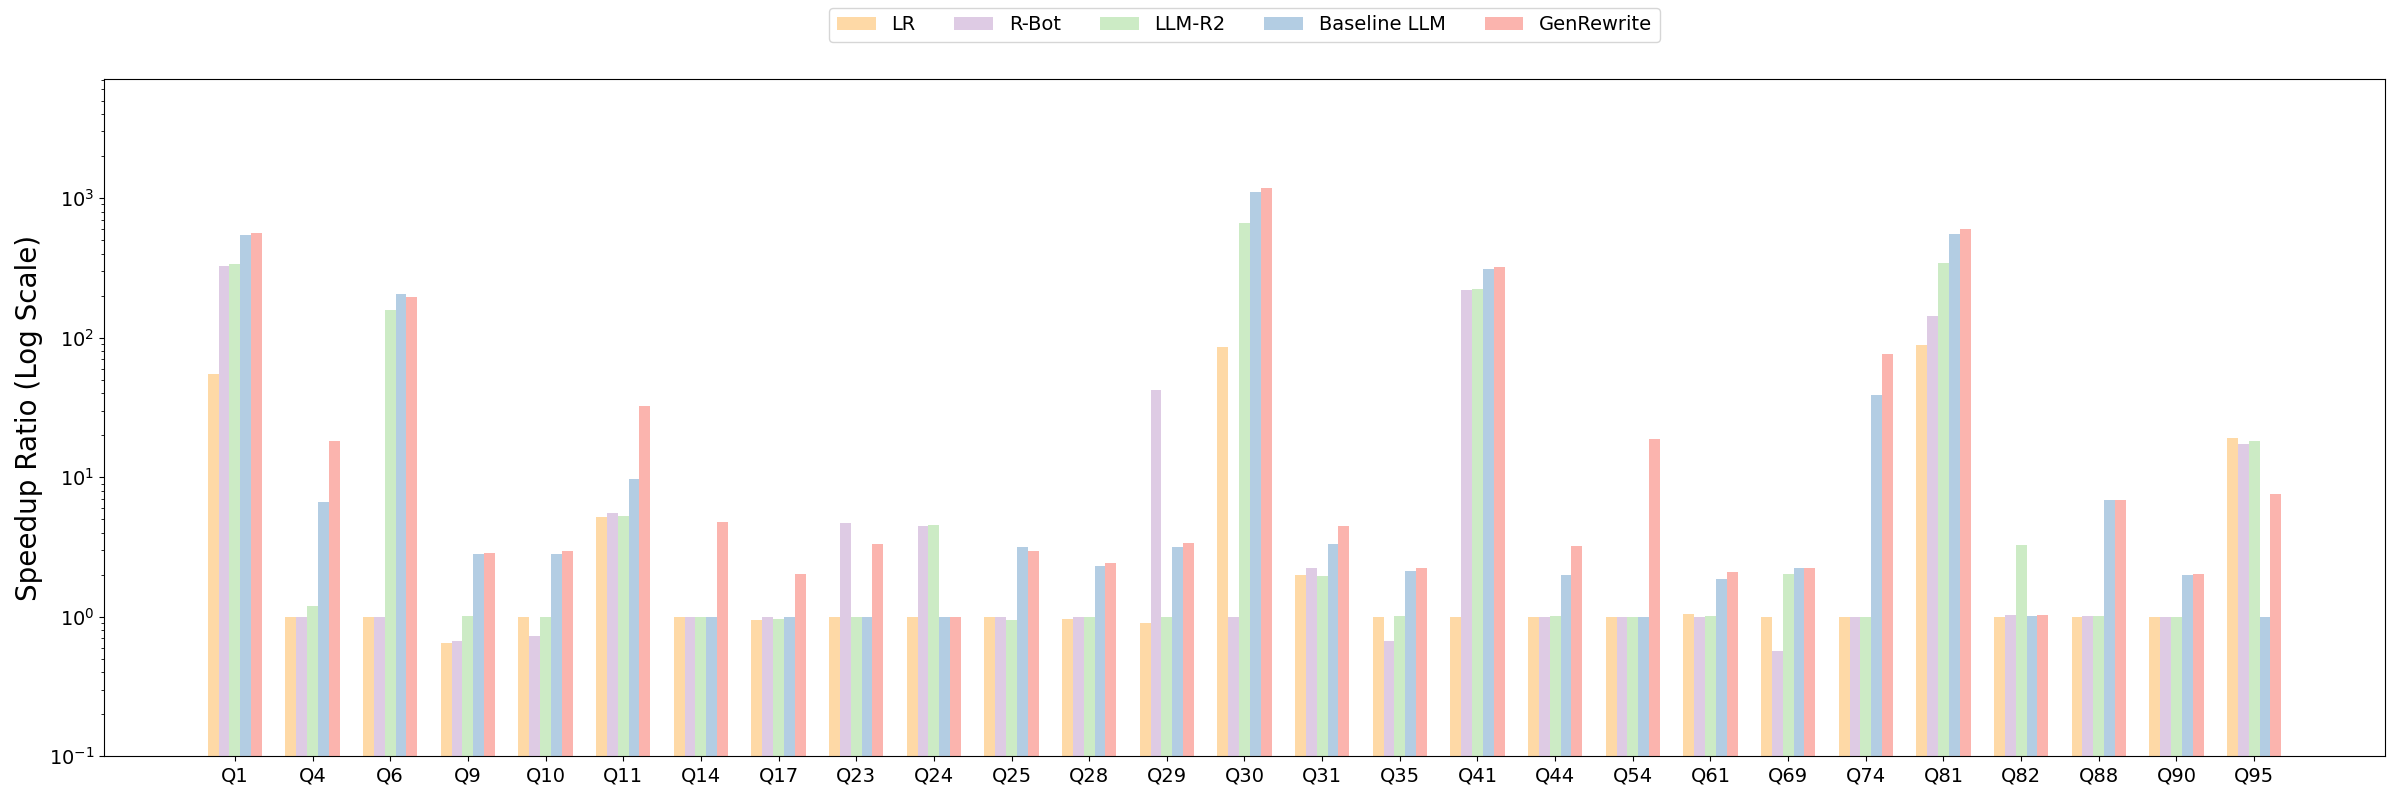
\includegraphics[width=\textwidth]{chapters/genrewrite/figures/baseline_comparison.png}
  \inv
  \vspace{-18pt}
  \captionsetup{font=small,name=Figure}
  \caption{Comparison of speedup achieved by different approaches on queries where at least one method attains a 2x or greater speedup. The y-axis is on a log scale.}
  \label{gen:fig:baseline}
  \inv
\end{figure*}

\end{comment}



\begin{comment}
    

In rule-based query rewriting, a set of pattern-matching rewrite rules define a fixed search space, resulting in consistent query outcomes across multiple runs. In contrast, due to the probabilistic nature of LLMs, 
    additional LLM runs increases the likelihood of uncovering new rewrite possibilities and thereby improving performance.
To ensure a fair comparison, we impose a limit on the number of LLM runs per query, 
    consistent with the setup outlined in Section~\ref{gen:sec:expr:llmbaseline}. Here, again, if a method fails to produce an equivalent rewrite for a particular query,  we deem the speedup ratio for that query as 1 indicating a fallback to the original query.
\end{comment}
% the number of iterations in \genrewrite to 5, including 4 i 
% a limit to the number LLM runs for each query in \genrewrite.

%  \genbarzan{check WA msg}
% \st{This predictability contrasts with the dynamic nature of LLM-based rewrites, where additional LLM runs increase the likelihood of uncovering new rewrite possibilities, potentially leading to significant performance boost.} 



% or if it is not applicable, \genbarzan{what does not applicable mean??}



\begin{comment}
    

\begin{table*}[h]
\centering
\begin{tabular}{lccccc}
\toprule
   & Syntax errors  & Semantic error & Regression (i.e., speedup < 1x) & >2x speedup \\
\midrule
\genrewrite & \textbf{4.3\%} &  \textbf{6.1\%}  & \textbf{2.0\%} & \textbf{21.2\%}  \\
Baseline LLM   & 30.3\%  & 29.3\% & 25.3\% & 10.1\% \\
\bottomrule
\end{tabular}
\caption{Comparison between \genrewrite and Baseline LLM on percentage of syntax error, syntax error, performance regression, more than 2x speedup}
\label{gen:tab:llmbaseline}
\end{table*}
\end{comment}


\subsection{Comparison with Rule-based Methods}
\label{gen:sec:expr:traditionalbaseline}


Analysis of Table.~\ref{gen:tab:speedup_all} shows that \genrewrite consistently surpasses the
three rule-based baselines in terms of the number of queries optimized, regardless of the desired speedup threshold, on all benchmarks. Other LLM-based methods also consistently outperform rule-based methods with smaller margins than \genrewrite.
We first consider the standard public benchmarks (Table~\ref{gen:tab:speedup_comparison}). On the original TPC-DS workload, \genrewrite identifies substantially more optimization opportunities than the rule-based baselines: it achieves at least 2x speedup on 25 queries, compared to 10, 9, and 6 queries for \textsc{LLM-R\textsuperscript{2}}, \rbot, and \lr, respectively. The advantage persists at higher thresholds (e.g., 10x speedup), and we observe a similar pattern on JOB. These results suggest that \genrewrite already outperforms established rule-based methods on well-studied public benchmarks.


\noindent\revtwo{SQLStorm workloads (Table~\ref{gen:tab:speedup_comparison_sqlstorm}) yield two key observations:}

\genhead{\revtwo{Observation 1}}
\revtwo{The performance gap between \genrewrite and the rule-based baselines widens on TPC-DS (SQLStorm).
    All three rule-based baselines (\textsc{LLM-R\textsuperscript{2}}, \rbot, and \lr) are built on top of Calcite and ultimately rely on Calcite’s rewrite rules. Their differences lie in rule selection and ordering, but they inherit the same two Calcite limitations: (1) \emph{Parser coverage:} The Calcite parser and validator do not fully support several constructs that appear in SQLStorm-generated  TPC-DS queries, such as recursive CTEs, \texttt{LENGTH}, etc. As a result, these systems only emit rewrites for roughly half of the input queries. (2) \emph{Rule coverage:} Even when Calcite can parse the query, its fixed rule set often fails to match the structure of these queries. SQLStorm's queries are not hand-polished benchmark SQL; they contain noisy nesting, ad hoc join predicates, and unseen operator combination that does not line up cleanly with Calcite’s stock transformations (e.g., predicate pushdown). In these cases, the systems may not show meaningful improvement. In contrast, \genrewrite does not depend on Calcite’s rule inventory. It can generate and iteratively refine rewrites for these same SQLStorm queries, which explains the widening gap on TPC-DS (SQLStorm).}

\genhead{\revtwo{Observation 2}}
\revtwo{On SQLStorm workloads, the ``LLM-enhanced'' rule-based systems degrade to the point that they can be outperformed by \lr, which does not use an LLM at all. \textsc{LLM-R\textsuperscript{2}} selects a few high-quality demonstration rewrites from a curated library using a learned retriever, and \rbot retrieves offline ``rewrite recipes'' mined from past queries. These strategies work on TPC-DS and JOB because the benchmark queries follow canonical patterns that are well represented in those demonstration pools. Under SQLStorm, however, the generated queries deviate substantially from those canonical patterns, so the retrieved demonstrations and recipes are often no longer relevant and provide poor guidance. \genrewrite, by contrast, is not limited to a static set of expert demonstrations or a fixed rule inventory. It employs iterative correction and accumulates transferable rewrite knowledge from prior queries, enabling it to adapt to new query forms without manual rule engineering.}



\revtwo{\genrewrite outperforms existing baselines both on the original TPC-DS / JOB benchmarks and on the SQLStorm-generated workloads. Its advantage becomes larger precisely in the regimes where fixed-rule systems provide poor coverage. If new rules were distilled from \genrewrite's successful rewrites on complex queries and then incorporated into Calcite, the rule-based methods could  be strengthened and extended to a broader class of queries.}



\genhead{\revtwo{A deeper look at rules discovered by \genrewrite}}
\revtwo{Besides standard Calcite rules (e.g., predicate pushdown, projection pruning), several papers propose more aggressive rewrite patterns for analytical workloads. Generalized Sub-Query Fusion~\cite{sarthi2020generalized} eliminates redundant I/O by fusing multiple similar subqueries into a single shared scan/aggregation. Super-operators~\cite{blitz2} collapse multi-branch aggregates and unions into a single streaming physical operator. The Spark engine in Azure Synapse~\cite{modi2021new} rewrites plans to reuse shuffles, push down filters and partial aggregates, and inject runtime partition pruning to reduce data movement. Athena~\cite{bruno2022computation} detects repeated expensive subplans in a query and fuses them so they are computed once and shared by all consumers. In Table~\ref{gen:tab:pattern-summary}, for each major rewrite pattern discovered by \genrewrite we ask: (1) does it align with any of these known patterns, at the idea level; and (2) is there an exact structural match already reported in prior work?}

% [leftmargin=0.5cm]

\noindent\revone{Representative optimization patterns discovered by \genrewrite:}
% \footnote{In Appendix~A, we present query pairs for each pattern and detail how they differ from prior work.}

\begin{enumerate}[leftmargin=0.5cm]
\item  \revone{Pivot with conditional aggregation instead of UNION-then-self-join.}
\item \revone{Replace multiple \texttt{EXISTS} conditions with a precomputed set via joins.}
\item \revone{Rewrite \texttt{COUNT(*)>0} as \texttt{EXISTS} (aggregate $\rightarrow$ semi-join; enables short-circuiting).}
\item \revone{Replace a bounded self-recursive CTE with a non-recursive base query \texttt{CROSS JOIN}ed to a small numbers table.}
\item \revone{Lift a per-key summary (e.g., item-level totals) into one CTE and drive all branches from it.}
\item \revone{Consolidate repetitive subqueries into a single aggregation subquery with conditional expressions.}
\item \revone{Decorrelate \texttt{IN} by joining a \texttt{SELECT DISTINCT} key,... mapping table instead of re-checking the subquery. }
\end{enumerate}


\begin{table}[tbp]
\inv
\small
\centering
\setlength{\tabcolsep}{6pt}
\def\arraystretch{1.2}

\begin{tabular}{ l | c c c }
\toprule
Pattern& Covered queries & Similar in idea & Exact match \\
\midrule
1 & 4, 11, 74 & ~\cite{blitz2}, ~\cite{bruno2022computation} & No \\
2 & 10, 35, 69 & ~\cite{begoli2018apache} & No \\
3 & 41 & ~\cite{begoli2018apache} & No \\
4 & 23998* &  & No \\
5 & 22722* & ~\cite{sarthi2020generalized}, ~\cite{bruno2022computation} & No \\
6 & 61, 88 & ~\cite{sarthi2020generalized}, ~\cite{bruno2022computation} & Yes,~\cite{bruno2022computation}  \\
7 & 28982*, 34389* & ~\cite{begoli2018apache} & Yes,~\cite{begoli2018apache}  \\
\bottomrule
\end{tabular}
\captionsetup{font=small,name=Table}
\caption{\revtwo{Summary of rewrite patterns discovered by \genrewrite. ``Covered queries'' lists the queries that exhibit each pattern (queries with * are from TPC-DS SQLStorm; others are from standard TPC-DS). ``Similar in idea'' notes prior work that proposes a conceptually related optimization. ``Exact match''indicates that the same structural rewrite has been reported before.}  }
\inv
\label{gen:tab:pattern-summary}
\end{table}











% \begin{enumerate}[leftmargin=0.5cm]

% \item  Pivot with conditional aggregation instead of UNION-then-self-join.
% \item Rewrite \texttt{COUNT(*)>0} as \texttt{EXISTS} (aggregate $\rightarrow$ semi-join; enables short-circuiting).
% \item Consolidate repetitive subqueries into a single aggregation subquery with conditional expressions.


% \end{enumerate}




\subsection{Detailed Analysis and Ablation Study}
\label{gen:sec:expr:ablation}

In this section, we conduct a detailed ablation study 
    to validate our design decisions in  \genrewrite and the contribution of each component therein towards the overall performance. We focus primarily on the \revtwo{original} TPC-DS benchmark, as its complexity provides a challenging test of our system's capabilities. The results, summarized in Table~\ref{gen:tab:ablation}, highlight the impact of individual components on LLM runtime overhead, monetary cost, and the percentage of queries achieving various levels of speedup.
    % To control for variables, we still adopt a setup in which our NLR2 repository is initialized with two LLM runs using the basic prompt and \genrewrite incorporates the NLR2 as a hint for the remaining two candidate rewrites,.


    




\begin{table*}[!t]
\small
\centering
\setlength{\tabcolsep}{5pt}
\def\arraystretch{1.1}
\vspace{-5pt}
\begin{tabular}{ | c | r r r r r |  }
\toprule
& \multicolumn{5}{c|}{TPC-DS} \\
 & >2x & >10x & >50x  & avg. time(s) & avg. cost(\$)  \\
\midrule
\genrewrite                           & \cntpct{25}{25.3} & \cntpct{9}{9.1}   & \cntpct{6}{6.1}   & 151.82 & 0.129 \\
\genrewrite without grouping NLR2s    & \cntpct{25}{25.3} & \cntpct{9}{9.1}   & \cntpct{6}{6.1}   & 385.47 & 0.310 \\
\genrewrite without bottleneck analysis & \cntpct{19}{19.2} & \cntpct{6}{6.1}   & \cntpct{5}{5.1}   & 150.30 & 0.124 \\
\genrewrite with gpt-4o               & \cntpct{14}{14.1} & \cntpct{5}{5.1}   & \cntpct{5}{5.1}   & 105.40 & 0.117 \\
\genrewrite with gpt-4-mini           & \cntpct{2}{2.0}   & \cntpct{1}{1.0}   & \cntpct{0}{0.0}   & 301.20 & 0.016 \\
\bottomrule
\end{tabular}
\captionsetup{font=small,name=Table}
\caption{Ablation study: impact of \genrewrite's design decisions on LLM runtime, cost, and the share of queries achieving various speedups.}
\label{gen:tab:ablation}
\vspace{-15pt}
\end{table*}



\genhead{Plan-based dominant NLR2 identification} This component plays a critical role in reducing query execution overhead, although its impact is not directly reflected in Table~\ref{gen:tab:ablation}. Without plan-based dominant NLR2 identification, we would need to execute each rewrite—generated by applying a single NLR2—to measure its runtime, which can be prohibitively expensive for long-running queries. 

\genhead{NLR2 grouping via LLM}
We collect an average of 5.08 NLR2s per input query after applying grouping, compared to 13.24 NLR2s per query without grouping. Although we only re-evaluate the impact of an NLR2 when the associated performance improvement exceeds a predefined threshold, grouping still significantly reduces both monetary and time costs. Without grouping, the average LLM runtime increases by 153.9\%, and the monetary cost rises by 140.3\%,  demonstrating that NLR2 grouping's impact on costs.


\genhead{Query performance bottleneck analysis} 
We compare two strategies: (1) apply the top NLR2s globally, ignoring query similarity; and (2) our default, which retrieves candidates by bottleneck similarity. The global strategy performs essentially the same as \baseline, indicating that ``best overall'' strategy rarely transfers. Bottleneck-aware retrieval, in contrast, delivers clear gains: effective reuse hinges on aligning NLR2s with performance bottlenecks.

% We evaluate two strategies for identifying queries with similar performance bottlenecks: (1) applying the top beneficial NLR2s regardless of query similarity, and (2) our default approach, which incorporates bottleneck-aware retrieval. Experimental results show that the first strategy performs nearly identically to \baseline, suggesting that indiscriminately applying high-performing NLR2s provides little benefit. This underscores the importance of relevance—effective reuse of NLR2s depends on accurately identifying queries with comparable performance bottlenecks.



\genhead{Choice of the LLM}
\genrewrite's performance critically depends on the LLM's reasoning capabilities. We evaluate three models: OpenAI’s \texttt{o3-mini} (reasoning-oriented), \texttt{gpt-4o} (balanced), and \texttt{gpt-4o-mini}(most cost-efficient).  \genrewrite powered by \texttt{gpt-4o} is noticeably outperformed by the \texttt{o3-mini} variant. We decompose \genrewrite’s workflow into two stages: (1) discovering effective rewrites and summarizing NLR2s, and (2) applying high-quality NLR2s to guide rewrites. We observe that \texttt{gpt-4o} struggles primarily in stage 1. However, when \genrewrite with \texttt{gpt-4o} is supplied with NLR2s previously discovered by \texttt{o3-mini}, the number of queries achieving a speedup $\geq$ 10× increases from 5 to 8,  further demonstrating the effectiveness of NLR2-guided rewriting.
% \texttt{gpt-4o-mini} rarely produces useful rewrites.



% \genrewrite’s gains track the model’s reasoning strength. \texttt{o3-mini} (reasoning-oriented) consistently finds stronger rewrites and better NLR2s, outperforming \texttt{gpt-4o}; \texttt{gpt-4o-mini} rarely produces useful rewrites. Decomposing \genrewrite into (i) discovery/summarization of NLR2s and (ii) application shows where the gap arises: \texttt{gpt-4o} underperforms in (i) but applies good NLR2s well—when seeded with \texttt{o3-mini}’s NLR2s, its count of >10× speedups rises from 5 to 8. Practical takeaway: use the strongest model for discovery, then a cheaper model can reliably apply the learned NLR2s.


\genhead{\revone{Parameter sensitivity analysis}}




\begin{table}[tbp]
\small
\centering
\begin{tabular}{l*{4}{cc}}
\toprule
& \multicolumn{2}{c}{$k{=}1$}
& \multicolumn{2}{c}{$k{=}2$}
& \multicolumn{2}{c}{$k{=}3$}
& \multicolumn{2}{c}{$k{=}4$} \\
\cmidrule(lr){2-3}
\cmidrule(lr){4-5}
\cmidrule(lr){6-7}
\cmidrule(lr){8-9}
& eq & fast
& eq & fast
& eq & fast
& eq & fast \\
\midrule
No correction
& 52 & 5
& 67 & 8
& 70 & 12
& 74 & 21 \\
Semantic only
& 54 & 5
& 68 & 10
& 71 & 14
& 75 & 21 \\
\textbf{Semantic + syntax}
& \textbf{70} & \textbf{5}
& \textbf{79} & \textbf{10}
& \textbf{85} & \textbf{16}
& \textbf{86} & \textbf{28} \\
\bottomrule
\end{tabular}
\captionsetup{font=small,name=Table}
\caption{\revone{Cumulative count of queries with (i) at least one equivalent rewrite (\textit{equiv}) and (ii) at least one equivalent rewrite that is at least 20\% faster than the original (\textit{faster}), as the candidate budget increases ($k{=}1\ldots4$), under different correction strategies.}}
\label{gen:tab:correction_ablation_new}
\inv
\end{table}


\noindent\revone{
\emph{\textbf{Budget:}} maximum candidates per query \(K=4\); correction caps \(I_{\mathrm{sem}}=I_{\mathrm{syn}}=3\) (semantic and syntax loops). For the TPC-DS workload, the average iterations is 0.30 (semantic) and 0.76 (syntax). The per-query correction iteration distributions are:}
\begin{itemize}
    \item \revone{Semantic: 0: 76.72\%, 1: 19.02\%, 2: 1.64\%, 3: 2.62\%.}
    \item \revone{Syntax: 0: 60.66\%, 1: 18.36\%, 2: 5.25\%, 3: 15.74\%.}
\end{itemize}
\revone{We vary the candidate budget $k \in\{1,2,3,4\}$. Table~\ref{gen:tab:correction_ablation_new} reports the \emph{cumulative} number of queries that achieve (i) $\geq 1$ equivalent rewrite and (ii) $\geq 1$ equivalent rewrite that is at least 20\% faster, as $k$ increases (higher \(k\) means more candidates attempted per input query), comparing: (i) no correction, (ii) semantic-only correction, and (iii) semantic\,+\,syntax correction.} \revone{Table~\ref{gen:tab:correction_ablation_new} shows that correction loops markedly reduce the effective error rate,  with \emph{semantic + syntax} outperforming the other settings at every \(k\). Larger \(k\) improves coverage with diminishing returns and proportionally higher cost.}


\noindent\revone{\emph{\textbf{Desired speedup threshold:}}
We set $\theta$ to 1.2x in our implementation. Increasing $\theta$ reduces coverage  but raises the average speedup among accepted rewrites. With a lower $\theta$, we keep more rewrites — including many that are only modestly better.}

\begin{table}[H]
\small
\centering
\begin{tabular}{lccc}
\toprule
Desired speedup threshold $\theta$ & 1.2x & 2.0x & 5.0x \\
\midrule
Coverage (\%)       & 28.3 & 23.2 & 13.1 \\
Geom.\ mean speedup & 11.1x & 17.0x & 72.2x \\
\bottomrule
\end{tabular}
\captionsetup{font=small,name=Table}
\caption{\revone{Coverage and geometric mean speedup for desirable speedup thresholds $\theta \in \{1.2x,1.5x,2.0x\}$. 
Coverage(\%) is the fraction of queries with $\ge\theta$ speedup; geom.\ mean is over covered queries.}}
\label{gen:tab:theta_sweep}
\inv
\end{table}

\vspace{-5mm}

\genhead{\revthree{Counterexample-guided iterative correction}} 
\revthree{We compare our counterexample-based semantic check to Miniature \& Mull from LLM-SQL-Solver~\cite{zhao2023llm} on random TPC-DS rewrites (no correction). Our prompt yields 29\% equivalent rewrites before syntax correction with a 6\% false-positive rate; Miniature \& Mull achieves 26\% equivalents with 22\% false positives. Thus our prompt better aligns with the iterative correction task—more verified equivalents and far fewer false positives.}



% \revthree{LLM-SQL-Solver~\cite{zhao2023llm} introduces the Miniature \& Mull prompting strategy for equivalence checking, which also searches for counterexamples and bases the decision on them. For a head-to-head comparison, we replaced our semantic-checking prompt with theirs and evaluated both settings on randomly sampled TPC-DS rewrites without any correction. With our prompt—which asks the LLM to produce a concrete counterexample and then feeds it back as a hint for semantic correction—we obtain 29\% equivalent rewrites \emph{before} syntax correction stage and a 6\% false-positive rate (inequivalent rewrites judged equivalent). Using Miniature \& Mull, we observe 26\% equivalent rewrites and a 22\% false-positive rate under the same protocol. This indicates our semantic-checking prompt is better aligned with the rewrite-correction loop, yielding more verified equivalents while substantially reducing false positives.}


% LLM-SQL-Solver proposes Miniature and Mull prompting technique for equivalence checking, which shares similar idea with our method about finding counterexamples and then give the conclusion. We replace our semantic checking prompt with theirs and test both on TPC-DS workloads. The result shows that with our semantic checking prompt which asks for a counterexample from LLMs and then be used as the hints for semantic corrections, we get 29\% equivalent queries (before syntax correction) and 6\%  false positive (LLMs consider the inequivalent rewrites to be equivalent). For LLM-SQL-Solver, we get 26\% equivalent queries and 22\% false positives. Our semantic checking prompt suits better with this rewrite correction task.














\begin{comment}


\genhead{Impact of semantic   and syntax correction} For each TPC-DS query, we conduct 4 independent runs to generate 4 candidate rewrites. In each run, we use zero-shot prompting (Baseline LLM) to suggest candidate queries and adopt one of the following correction strategies before assessing the correctness and performance of the rewrite.

\begin{enumerate}
    \item No correction.
    \item Only semantic correction.
    \item Only syntactic correction.
    \item Two-stage correction (semantic correction and then syntax correction).
\end{enumerate}



\noindent We set the maximum iteration count 3 for both semantic and syntax correction.

Table~\ref{gen:tab:correction_ablation} compares cumulative equivalent rewrites generated by various correction strategies over successive runs, with each cell showing the number of TPC-DS queries equivalently rewritten by a specific strategy up to that point (the highest possible is 99). The analysis clearly demonstrates that the two-stage correction strategy outperforms others, and not applying any correction yields the least effective results, with the remaining strategies falling in between. In a direct comparison between ``Only semantic correction'' and ``Only syntax correction'', the latter shows a quicker ability to produce executable and equivalent rewrites for simpler queries in the first few runs. However, its effectiveness is limited by a lower ceiling due to a lack of understanding regarding the queries' intent, leading to executable but inequivalent rewrites for more complex queries. When combining these two strategies together, semantic correction interprets the intent, ensuring the rewrite's objectives align with the original query, and then syntax correction refines the rewrite to be executable. The two-stage strategy (i.e., semantic + syntax) identifies equivalent rewrites for 70 of the 99 TPC-DS queries in the first run. It then adds 3 more in the second run and 6 in the third, ultimately achieving equivalent rewrites for 90 of the 99 queries.



\begin{table}[h]
\centering
\begin{tabular}{lcccc}
\toprule
 & run 1 & run 2 & run 3 & run 4 \\
\midrule
No correction & 45 & 56 & 65 & 69  \\
Only semantic & 51 & 66 & 76 & 82 \\
Only syntactic & 60 & 68 & 73 & 76 \\
\textbf{Semantic + syntactic} & \textbf{70} & \textbf{81} & \textbf{87} & \textbf{90} \\
\bottomrule
\end{tabular}
\caption{Cumulative count of equivalent rewrites   using different correction strategies over multiple runs.}
\label{gen:tab:correction_ablation}
\inv
\end{table}



Delving deeper into the two-stage correction strategy, it generally achieves convergence quickly, usually within 3 iterations, except for a small number of cases involving overly complex queries. However, there is still a gap between the queries deemed equivalent by the LLM and those that are truly equivalent. The non-cumulative count of queries  verified as equivalent in each run are 69, 75, 69, and 70, respectively.  When aggregating results from all runs, 90 unique queries are   equivalent, indicating that the sets of queries identified as equivalent in each run vary.




    

\genhead{Impact of NLR2s as hints}  After conducting 4 rounds of zero-shot prompting, we reach a stable state where additional rounds fail to bring improvements in terms of the number of rewrites that are both equivalent and faster.
This suggests that we effectively capture most of low-hanging fruits. A comparative analysis between an additional iteration using zero-shot prompting and another leveraging prompts augmented with specific NLR2 hints reveals a pronounced superiority of the latter. The queries solvable exclusively through hint-augmented prompts 
are presented in Table~\ref{gen:tab:knowledge_ablation}.


% Two crucial observations are highlighted in Section 3: LLMs are more likely to struggle in identifying rewrite opportunities with increasing query complexity; LLMs can optimize queries that they previously struggled to optimize when provided with suitable hints in the prompt. The primary goal of employing NLR2s is to facilitate knowledge transfer and bridge the gap between queries that LLMs can optimize without hints and those they cannot, enabling LLMs to optimize a broader range of queries.

% \begin{table}[ht]
% \centering
% \caption{Rewrite hints .}
% \label{gen:tab:knowledge_ablation}
% \begin{tabular}{lccccc}
% \toprule
%  & Q4 & Q11 & Q20 & Q29 & Q76 \\
% \midrule
% Without hints & - & 1.07x & 1x & 1.42x & 1x  \\
% With hints & \textbf{5.68x} & \textbf{10.3x} & \textbf{9.89x} & \textbf{6.85x} & \textbf{9.77x} \\
% \bottomrule
% \end{tabular}
% \end{table}


% \begin{table}[h]
% \centering
% \caption{NLR2s inspired speedups}
% \label{gen:tab:knowledge_ablation}
% \begin{tabular}{ccc p{4cm}}
% \toprule
% input & speedup & inspired by & \small{NLR2s} \\
% \hline
% 4 & 5.68x & 74 &  \footnotesize{Avoid UNION ALL if not necessary \newline Split complex queries into simpler ones using WITH clause} \\ \hline
% 11 & 10.3x & 74 & \footnotesize{Avoid UNION ALL if not necessary \newline Split complex queries into simpler ones using WITH clause} \\ \hline
% 20 & 9.89x & 12 &  \footnotesize{Use CTE (Common Table Expressions) to break down complex queries \newline Reduce the number of tables in the join operation} \\ \hline
% 29 & 6.85x & 25 &  \footnotesize{Aggregate before join \newline Use subqueries to break down complex queries} \\ \hline
% 76 & 9.77x & 61 &  \footnotesize{Combine multiple queries into a single query \newline Move WHERE clause filters to ON clause in JOINs} \\
% \bottomrule
% \end{tabular}
% \end{table}





Q4, Q11, and Q74 all see improvements by eliminating the unnecessary \sqlunionallcolor, which has been discussed in earlier sections. Q20 benefits from NLR2s learned from its neighboring query Q12. Inspired by the rule ``Use CTE to break down complex queries'', the actual transformation applied is a group-by pushdown. Q29 is solved using similar ideas but exhibits a different query pattern and learns from Q25.
For Q76,  where multiple segments each join two common tables across several subqueries, the rewrite strategy is to combine these segments with \sqlunionallcolor before conducting a join with the common tables, thereby avoiding duplicate computation. This strategy is inspired by the rule ``Combine multiple queries into one query'' from Q61. These instances underscore the value of employing NLR2s for effective knowledge transfer across queries. At the conclusion of our experiments, we collect 156 groups of rewrite rules,  with an average of 7 rules per group.
\end{comment}

\begin{comment}
    

\genhead{\texttt{EXPLAIN} cost vs. actual latency} When evaluating rewrites, we can either utilize the database's own cost estimates as a surrogate for actual performance (i.e., using \texttt{EXPLAIN}) 
or measure the latency by actually running candidate queries directly on the database or a small sample of it. The latter approach, while offering greater accuracy, also results in higher costs, which is justifiable when the query is optimized once and rewritten many times (see target use case in \S\ref{gen:sec:intro}). The goal of this experiment is to quantify the negative impact of using 
inaccurate cost estimates on \genrewrite's performance.

We examine two variants of \genrewrite, differing only in their choice of evaluation metric. One variant calculates the utility scores of NLR2s   based on actual latency while the other relies on \texttt{EXPLAIN}'s cost estimates. 
The comparison between the two variants is detailed in 
Table~\ref{gen:tab:latency_vs_cost}. We observe that both coverage and latency reduction ratios are lower when \texttt{EXPLAIN} is used for query evaluation. This is expected: (1) cost estimates do not accurately reflect actual latency, meaning a rewrite with a lower cost estimate does not guarantee lower latency; (2) the speedup ratios derived from cost estimates can be disproportionately high, not aligning with the actual latency improvements, thereby impacting the effectiveness of NLR2s. Despite these issues, the variant that rely on \texttt{EXPLAIN} cost still outperforms all other baselines.

\end{comment}








\subsection{Time and Monetary Cost}
% \subsection{Cost analysis of LLM}
\label{gen:sec:expr:llmcost}


While \genrewrite’s time and API costs are a one-time, amortized expense for recurring workloads (see Target workloads in \S\ref{gen:sec:intro}), we still quantify them to ensure they remain modest. Using OpenAI’s \texttt{o3-mini} to generate a rewrite for a TPC-DS query—including suggestion, semantic correction, and syntactic correction—costs on average \$0.029 and takes 36.15 s. For comparison, \texttt{gpt-4o} and \texttt{gpt-4o-mini} average (\$0.026, 25.1 s) and (\$0.004, 71.71 s), respectively. As a reasoning-focused model, \texttt{o3-mini} consumes more tokens, increasing cost but often yielding more logically sound, well-structured rewrites for complex SQL transformations. Auxiliary LLM steps (e.g., grouping NLR2s and selecting the bottleneck) add negligible overhead. Overall, total cost scales approximately linearly with the number of candidate rewrites generated by the pipeline.


%  Although the time and monetary cost of \genrewrite is not as relevant given that it is a one-time cost that gets amortized for recurrent workloads (see Target workloads in \S\ref{gen:sec:intro}), we still need to ensure they do not become excessive.
% Using OpenAI’s \texttt{o3-mini} model to generate a rewrite for a TPC-DS query—including rewrite suggestion, semantic correction, and syntactic correction—incurs an average cost of approximately \$0.029 and takes 36.15 seconds. For comparison, \texttt{gpt-4o} and \texttt{gpt-4o-mini} yield average costs and durations of (\$0.026, 25.1 seconds) and (\$0.004, 71.71 seconds), respectively. \texttt{o3-mini}, being a reasoning-focused model, tends to consume significantly more tokens during generation. While this leads to higher total costs, the increased token usage contributes to more logically sound and well-structured rewrites, especially in the context of complex SQL transformation tasks.
% The cost associated with auxiliary LLM tasks, such as grouping NLR2s and selecting the most relevant bottleneck  is negligible in practice. Overall, the total cost of the system grows linearly with the number of candidates generated with the rewriting pipeline.


% Although \texttt{gpt-4o} is approximately twice as expensive per token as \texttt{o3-mini}, and roughly 16 times more expensive than \texttt{gpt-4o-mini}, our experiments show that the overall cost of using \texttt{o3-mini} is actually higher than that of \texttt{gpt-4o}. This counterintuitive result stems from the fact that \texttt{o3-mini}, being a reasoning-focused model, tends to consume significantly more tokens during generation. While this leads to higher total costs, the increased token usage contributes to more logically sound and well-structured rewrites, especially in the context of complex SQL transformation tasks.
% The cost associated with auxiliary LLM tasks, such as grouping NLR2s and selecting the most relevant bottleneck from the top-$k$ candidates—is negligible in practice. Overall, the total cost of the system grows linearly with the number of iterations of the rewriting pipeline.



\begin{table}[h]
% \small
\footnotesize
\centering
\setlength{\tabcolsep}{6pt}
\def\arraystretch{1.1}
\vspace{-5pt}
\begin{tabular}{  c | r r r | r r r }
\toprule
& \multicolumn{3}{c|}{time (s)} 
& \multicolumn{3}{c}{monetary cost (\$)} \\
stage & suggest & \makecell{semantic\\corr.} & \makecell{syntax\\corr.} & suggest & \makecell{semantic\\corr.} & \makecell{syntax\\corr.} \\
\midrule
o3-mini     & \makecell{5.8\\(16.0\%)} & \makecell{20.8\\(57.6\%)}  & \makecell{9.6\\(26.5\%)}  & \makecell{7.8e-03\\(26.4\%)} & \makecell{1.5e-02\\(52.2\%)}  & \makecell{6.3e-03\\(21.3\%)} \\
gpt-4o & \makecell{1.5\\(5.8\%)} & \makecell{22.1\\(87.9\%)}  & \makecell{1.6\\(6.3\%)}  & \makecell{6.4e-03\\(23.9\%)} & \makecell{1.9e-02\\(70.1\%)}  & \makecell{1.6e-03\\(6.0\%)} \\
gpt-4o-mini & \makecell{1.9\\(2.6\%)} & \makecell{66.8\\(93.1\%)}  & \makecell{3.1\\(4.3\%)}  & \makecell{4.0e-04\\(11.2\%)}  & \makecell{3.1e-03\\(84.6\%)}   & \makecell{1.5e-04\\(4.2\%)} \\
% \rbot       & \makecell{9\\(9.1\%)}  & \makecell{5\\(5.1\%)}   & \makecell{3\\(3.0\%)}   & \makecell{7\\(6.2\%)}  & \makecell{3\\(2.7\%)}   & \makecell{2\\(1.8\%)} \\
% \lr       & \makecell{6\\(6.1\%)}  & \makecell{4\\(4.0\%)}   & \makecell{0\\(0\%)}   & \makecell{6\\(5.3\%)}  & \makecell{2\\(1.8\%)}   & \makecell{1\\(0.9\%)} \\
\bottomrule
\end{tabular}
\captionsetup{font=small,name=Table}
\caption{\small LLM cost analysis: the monetary and time cost of generating one rewrite candidate for a TPC-DS query, including all three stages--- rewrite suggestions, semantic correction, and syntactic correction.}
\inv
\label{gen:tab:llm_cost}
\vspace{-10pt}
\end{table}

 
 % The breakdown of the monetary and time cost is presented in Table~\ref{gen:tab:llm_cost}. Across all three models, semantic correction phase accounts for the highest cost in terms of both monetary and time cost. However, when using \texttt{o3-mini}, a larger portion of time is also spent on the candidate suggestion and syntax correction phases. This is because \texttt{o3-mini}, with its stronger reasoning capabilities, tends to better understand the input query and generate more aggressive rewrites. While this increases the likelihood of discovering high-quality transformations, it also lowers the chance of producing equivalent rewrites on the first attempt, thereby requiring additional iterations in the syntax correction phase. In contrast, the two lower-capacity models exhibit a more conservative rewriting style, leading to fewer iterations but also fewer opportunities for substantial performance improvement.

 Table~\ref{gen:tab:llm_cost} shows that semantic correction dominates both time and cost across models. With \texttt{o3-mini}, more time also goes to candidate suggestion and syntax correction: its stronger reasoning yields more aggressive rewrites (more chances for big wins) but requires extra iterations to ensure equivalence. By contrast, \texttt{gpt-4o} and \texttt{gpt-4o-mini} rewrite more conservatively, needing fewer iterations but offering fewer opportunities for substantial speedups.

\revone{For equivalence checking, we set a 60 sec timeout for the tester and 5 sec for the verifier. Performance–evaluation time varied by query from seconds to hours. We also terminated execution early when a candidate failed to exceed the original query by the desired speedup threshold $\theta$.}

 


% \subsection{Choice of the LLM}
% \label{gen:sec:expr:llmchoice}

% The performance of components in \genrewrite critically depends on the knowledge and reasoning capabilities of the chosen LLM. If an LLM fails to optimize queries, no transferable knowledge is generated, and if it does not accurately capture a query’s objective, it is unlikely to identify relevant counterexamples. We evaluate three LLMs with varying costs and capabilities: OPENAI o3-mini, which excels at reasoning; gpt-4, the state-of-the-art general-purpose model; and gpt-3.5-turbo, which provides basic text understanding. As shown in Table~\ref{gen:tab:ablation}, OPENAI o3-mini achieves the best speedup statistics at a modest cost, demonstrating both the rapid progress in language models for complex tasks and the powerful reasoning capabilities even in small-scale models.





% \genhead{LLM's capacity}






% evaluating queries with explain costs or actual latency


% \noindent\textbf{Compared approaches.} To understand the contribution of various components within our tool, we remove certain components to compare its performance with that of the complete tool.

% \begin{itemize}
%     \item \textbf{Zero-shot prompts with no correction.}
%     \item \textbf{Zero-shot prompts with only semantic correction.}
%     \item \textbf{Zero-shot prompts with only syntax correction.}
%     \item \textbf{Zero-shot prompts with two-stage correction.}
%     \item \textbf{Prompts with rewrite hints (\texttt{EXPLAIN} cost).}
%     \item \textbf{Prompts with rewrite hints (actual latency).}
%     \item \textbf{}
%     \item 
    
% \end{itemize}



\begin{comment}
    
\begin{table}[!t]
\small
\centering
\setlength{\tabcolsep}{6pt}
\def\arraystretch{1.1}

\vspace{-5pt}
\begin{tabular}{  c | r r r | r r r }
\toprule
& \multicolumn{3}{c|}{TPC-DS} 
& \multicolumn{3}{c}{JOB} 
%& \multicolumn{2}{c|}{TPC-H} 
%& \multicolumn{2}{c}{TPC-DS} 
\\ 
speedup & >2x 
& >10x
& >50x 
& >1.2x 
& >2x
& >10x 
%& median 
%& max 
%& median 
%& max 
\\ 
\midrule
\genrewrite
& {25} & {9} & 
 {6}	&  {24}	& 8
& 3 
 %& \ruirevisiontbd{4.15}  &  \ruirevisiontbd{4.58}	 &  \ruirevisiontbd{5.03}		& \ruirevisiontbd{5.74}
\\ 
\baseline
& 18 & 6 & 5	& 19	 & 7
& 3 
%& 0.25 & 	1.58 & 	2.48	& 25.51 
\\ 
\textbf{LLM-R\textsuperscript{2}}
& 10	& 6 &	5	& 9	& 2
& 1 
%& 0.36	& 0.36	& NA &	NA 
\\ 
\lr
& 6	& 4 &	0	& 6	& 2
& 1
%& 0.36	& 0.36	& NA &	NA 
\\ 

\bottomrule
\end{tabular}
\caption{\small Speedup.}
\label{gen:tab:f}
\vspace{-15pt}
\end{table}
\end{comment}



\begin{comment}
    Since LLMs operate probabilistically, more trials increase the chances of finding a better rewrite. However, this is impractical due to time and cost constraints. Therefore, a system that more effectively uncovers hidden rewrite opportunities can significantly reduce both computational expenses and execution time.

From Table~\ref{gen:speedup_comparison}, we could see that both LLM-based 
which could be easily explained as LLMs have accumulated a solid knowledge base from the massive training data

\end{comment}


\begin{comment}
     Table~\ref{gen:tab:llmbaseline} shows a direct comparison between \genrewrite and  Baseline LLM. 
Notably, 30.3\% of  Baseline LLM's rewrites  are unexecutable (due to syntax error), compared to only 4.3\% for \genrewrite. The percentage of rewrites leading to semantic errors (i.e., non-equivalent rewrites) for Baseline LLM is 29.3\%, compared to only 6.1\% for \genrewrite. Both results demonstrate the effectiveness of our iterative correction strategy.


%marginally higher than BaselineLLM's 18.7\%, a result that initially appears surprising. In fact, it does not imply that \genrewrite's syntax correction is useful while its semantic correction is flawed. An unexecutable rewrite may indicate either a syntax error or both syntax and semantic errors, meaning SemanE does not accurately capture the ratio of semantic errors. A significant portion of SynE also has semantic errors.

\genrewrite results in only 2 performance regressions from 93 queries with equivalent rewrites-—-defined as those with over 5\% longer execution time than the original query--—while Baseline LLM experiences 23 performance regressions out of 70 equivalent rewrites. Moreover, \genrewrite achieves more than a 2x speedup in its rewrites twice as often as Baseline LLM. There two statistics show the effectiveness of our knowledge transfer.

% \genrewrite has a 25\% chance of generating incorrect queries, significantly lower than Baseline LLM's 49\%. Consequently, \genrewrite can produce equivalent rewrites for 93.9\% of TPC-DS queries, compared to Baseline LLM's 70.7\%. When selecting the best rewrites for comparison with the input queries, 

Overall, these results show the effectiveness of \genrewrite in drastically improving the quantity and quality of rewrites that one can achieve by na\"ively invoking the LLM.


Separate evaluation of NLR2s not only identify the exact contribution of each NLR2 but also find the NLR2 that leads to inequivalence. For example

\end{comment}


\begin{comment}
    
\begin{table}[tb]
\centering
\begin{tabular}{lccccc}
\toprule
speedup & >10\% & >50\% & >2x & >10x & >100x \\
\midrule
Using latency & \textbf{33.3\%} & \textbf{24.2\%} & \textbf{21.2\%} & \textbf{9.1\%} & \textbf{3.0\%} \\
Using \texttt{EXPLAIN} cost & 23.2\% & 16.2\% & 13.1\% & 7.1\% & \textbf{3.0\%} \\
\bottomrule
\end{tabular}
\caption{Comparison of the percentage of queries optimized when using latency and \texttt{EXPLAIN} cost as the evaluation metric}
\label{gen:tab:latency_vs_cost}
\inv
\end{table}
\end{comment}



\begin{comment}
    \begin{table}[tb]
\inv
\centering
\setlength{\tabcolsep}{3pt} % Adjust the space between columns
\begin{tabular}{@{}cccp{4.5cm}@{}}
\toprule
input & speedup & inspired by & \small{NLR2s} \\
\midrule
Q4 & 5.68x & Q74 &  \footnotesize{Avoid UNION ALL if not necessary; \newline Split complex queries into simpler ones using WITH clause} \\
Q11 & 10.3x & Q74 & \footnotesize{Avoid UNION ALL if not necessary; \newline Split complex queries into simpler ones using WITH clause} \\
Q20 & 9.89x & Q12 &  \footnotesize{Use CTE (Common Table Expressions) to break down complex queries; \newline Reduce the number of tables in the join operation} \\
Q29 & 6.85x & Q25 &  \footnotesize{Aggregate before join; \newline Use subqueries to break down complex queries} \\
Q76 & 9.77x & Q61 &  \footnotesize{Combine multiple queries into a single query; \newline Move WHERE clause filters to ON clause in JOINs} \\
\bottomrule
\end{tabular}
\caption{NLR2s inspired speedups}
\label{gen:tab:knowledge_ablation}
\inv
\end{table}
\end{comment}


\begin{comment}
    \begin{table}[H]
\small
\centering
\begin{tabular}{lcccc}
\toprule
 & \(k{=}1\) & \(k{=}2\) & \(k{=}3\) & \(k{=}4\) \\
\midrule
No correction & 52 & 67 & 70 & 74 \\
Semantic only & 54 & 68 & 71 & 75 \\
\textbf{Semantic + syntax} & \textbf{70} & \textbf{79} & \textbf{85} & \textbf{86} \\
\bottomrule
\end{tabular}
\captionsetup{font=small,name=Table}
\caption{Cumulative count of queries with $\geq$1 equivalent rewrites as the candidate budget increases (\(k=1\ldots 4\)), under different correction strategies.}
\label{gen:tab:correction_ablation}
\inv
\end{table}
\end{comment}




\begin{comment}


\begin{table}[H]
\small
\centering
\setlength{\tabcolsep}{6pt}
\def\arraystretch{1.1}
\vspace{-5pt}
\begin{tabular}{  c | r r r | r r r }
\toprule
& \multicolumn{3}{c|}{TPC-DS} 
& \multicolumn{3}{c}{JOB} \\
speedup & >2x & >10x & >50x & >1.2x & >2x & >10x \\
\midrule
\genrewrite     & \makecell{25\\(25.3\%)} & \makecell{9\\(9.1\%)}  & \makecell{6\\(6.1\%)}  & \makecell{20\\(17.7\%)} & \makecell{8\\(7.1\%)}  & \makecell{3\\(2.7\%)} \\
\baseline & \makecell{18\\(18.2\%)} & \makecell{6\\(6.1\%)}  & \makecell{5\\(5.1\%)}  & \makecell{19\\(16.9\%)} & \makecell{7\\(6.2\%)}  & \makecell{3\\(2.7\%)} \\
\lithe & \makecell{16\\(x\%)} & \makecell{6\\(6.1\%)}  & \makecell{4\\(x\%)}  & \makecell{17\\(x\%)} & \makecell{6\\(x\%)}  & \makecell{1\\(x\%)} \\
\textsc{LLM-R\textsuperscript{2}} & \makecell{10\\(10.1\%)} & \makecell{6\\(6.1\%)}  & \makecell{5\\(5.1\%)}  & \makecell{9\\(8.0\%)}  & \makecell{2\\(1.8\%)}   & \makecell{1\\(0.9\%)} \\
\rbot       & \makecell{9\\(9.1\%)}  & \makecell{5\\(5.1\%)}   & \makecell{3\\(3.0\%)}   & \makecell{7\\(6.2\%)}  & \makecell{3\\(2.7\%)}   & \makecell{2\\(1.8\%)} \\
\lr       & \makecell{6\\(6.1\%)}  & \makecell{4\\(4.0\%)}   & \makecell{0\\(0\%)}   & \makecell{6\\(5.3\%)}  & \makecell{2\\(1.8\%)}   & \makecell{1\\(0.9\%)} \\
\bottomrule
\end{tabular}
\captionsetup{font=small,name=Table}
\caption{Speedup Comparison between all methods on original TPCDS and JOB workloads.}
\label{gen:tab:speedup_comparison}
\vspace{-15pt}
\end{table}



\begin{table}[H]
\small
\centering
\setlength{\tabcolsep}{6pt}
\def\arraystretch{1.1}
\vspace{-5pt}
\begin{tabular}{  c | r r r | r r r }
\toprule
& \multicolumn{3}{c|}{TPC-DS (SQLStorm)} 
& \multicolumn{3}{c}{JOB (SQLStorm)} \\
speedup & >2x & >10x & >50x & >1.2x & >2x & >10x \\
\midrule
\genrewrite     & \makecell{25\\(25.3\%)} & \makecell{9\\(9.1\%)}  & \makecell{6\\(6.1\%)}  & \makecell{20\\(17.7\%)} & \makecell{8\\(7.1\%)}  & \makecell{3\\(2.7\%)} \\
\baseline & \makecell{18\\(18.2\%)} & \makecell{6\\(6.1\%)}  & \makecell{5\\(5.1\%)}  & \makecell{19\\(16.9\%)} & \makecell{7\\(6.2\%)}  & \makecell{3\\(2.7\%)} \\
\lithe & \makecell{16\\(x\%)} & \makecell{6\\(6.1\%)}  & \makecell{4\\(x\%)}  & \makecell{17\\(x\%)} & \makecell{6\\(x\%)}  & \makecell{1\\(x\%)} \\
\textsc{LLM-R\textsuperscript{2}} & \makecell{10\\(10.1\%)} & \makecell{6\\(6.1\%)}  & \makecell{5\\(5.1\%)}  & \makecell{9\\(8.0\%)}  & \makecell{2\\(1.8\%)}   & \makecell{1\\(0.9\%)} \\
\rbot       & \makecell{9\\(9.1\%)}  & \makecell{5\\(5.1\%)}   & \makecell{3\\(3.0\%)}   & \makecell{7\\(6.2\%)}  & \makecell{3\\(2.7\%)}   & \makecell{2\\(1.8\%)} \\
\lr       & \makecell{6\\(6.1\%)}  & \makecell{4\\(4.0\%)}   & \makecell{0\\(0\%)}   & \makecell{6\\(5.3\%)}  & \makecell{2\\(1.8\%)}   & \makecell{1\\(0.9\%)} \\
\bottomrule
\end{tabular}
\captionsetup{font=small,name=Table}
\caption{Speedup Comparison between all methods on original TPCDS and JOB workloads.}
\label{gen:tab:speedup_comparison_sqlstorm}
\vspace{-15pt}
\end{table}
    
\end{comment}


\begin{comment}

\item \textbf{TPC-DS} is a widely recognized, industry-standard decision support benchmark.
% , which is designed to provide relevant, objective performance data to industry users
 Even though
TPC-DS may not perfectly model the recurring workloads seen in production environments, it still serves as a valuable reference for assessing the efficacy of different query rewriting techniques on complex, real-life queries. We generated 
a 10GB TPC-DS dataset and considered all of the 99 queries in the benchmark. 

\item \textbf{JOB}~\cite{leis2015good} which is based on the IMDB data set, is a widely adopted test suite used to evaluate query optimization strategies in relational database systems. It consists of queries with varying degrees of complexity and multiple join operations, reflecting realistic workloads.

\item \textbf{TPC-DS (SQLStorm)} SQLStorm generates tens of thousands of queries using TPC-DS schema. Since calling LLM API incurs cost, it is not practical to test against all of them. We selected top 100 queries having the longest running time when testing using olapbench. All of the selected queries are of medium to high complexity based on SQLStorm's analysis.

\item \textbf{JOB (SQLStorm)} Similar to TPC-DS (SQLStorm), we also selected top 50 queries having the longest running time when testing using olapbench. All of the selected queries are of medium to high complexity based on SQLStorm's analysis.

    
\end{comment}


\begin{comment}

\revone{Table~\ref{gen:tab:speedup_all} presents the speedup comparison beween all methods. Before going into details, note that no matter it is the original workloads or SQLStorm-generated variants, queries in the JOB benchmark tend to be less complex compared to TPC-DS. First, the average query length in JOB is 278.81 tokens, while TPC-DS queries average 441.34 tokens—a 58\% increase. Second, although JOB queries can involve many joins and may present a combinatorial challenge in terms of finding the optimal join sequence, their structural complexity is lower: they feature fewer nested subqueries, window functions, and set operations than TPC-DS queries. When SQLStorm generates queries for TPC-DS and JOB schemas, JOB queries are still limited by the relatively narrow and normalized tables and lack of comparisons across channels or time windows } 
    
\end{comment}


% or if it is not applicable, \genbarzan{what does not applicable even mean?}


% \genrewrite & \textbf{4.3\%} &  \textbf{6.1\%}  & \textbf{2.0\%} & \textbf{21.2\%}  \\
% Baseline LLM   & 30.3\%  & 29.3\% & 25.3\% & 10.1\% \\

% Both \genrewrite and \baseline are given four attempts to propose candidate rewrites for each input query. 

% Table.~\ref{gen:tab:speedup_all} reports the percentage by dividing the number of queries by the total number of input queries, 99 for TPC-DS and 113 for JOB.


\cut{
\lr~\cite{LR} and \textsc{LLM-R\textsuperscript{2}}~\cite{li2024llm} both integrate
Apache Calcite~\cite{begoli2018apache} as the underlying rewrite engine and learn to select from Calcite’s rewrite rules to maximize their benefits. Nonetheless, their ability to rewrite SQL queries is inherently limited by the scope and expressiveness of Calcite's rule set.}






\begin{comment}
    

First, the gap between \genrewrite and the rule-based baselines widens on TPC-DS (SQLStorm). All three rule-based baselines (\textsc{LLM-R\textsuperscript{2}}, \rbot, and \lr) are built on top of the same Calcite rewriting engine. They differ mainly in how they choose which Calcite rule to apply and in what sequence, but they still depend on Calcite’s fixed rule set.



From Table.~\ref{gen:tab:speedup_comparison}, we can see that \genrewrite clearly outperforms rule-based methods by large margins on standard public benchmarks. On the original TPC-DS benchmark, \genrewrite improves 25 queries to achieve at least a 2× speedup, compared to 10, 9, and 6 queries optimized to the same level by \textsc{LLM-R\textsuperscript{2}}, \rbot, and \lr, respectively. For the more stringent 10× speedup threshold, \genrewrite again leads with 9 optimized queries, while \textsc{LLM-R\textsuperscript{2}}, \rbot, and \lr achieve 6, 5, and 4 queries, respectively. Similar trends hold for the JOB benchmark. \genrewrite optimizes 8 queries out of 113 queries to a 10× speedup, whereas \textsc{LLM-R\textsuperscript{2}}, \rbot, and \lr optimize only 2, 3, and 2 queries, respectively. 

From Table.~\ref{gen:tab:speedup_comparison_sqlstorm}, we have two interesting observations: 

observation 1 there is a even larger gap between \genrewrite and rule-based methods in TPC-DS SQLStorm variant than original TPC-DS. these three rule-based methods all use Calcite rewriter as the backbone. They are using the same fixed set of Calcite rewrite rules. The difference is which rule to use and in which order to apply selected rules. Therefore, they all suffer if Calcite cannot parse incoming queries or the incoming query patterns are too complex to be matched to existing calcite rules.
TPC-DS queries generated by SQLStorm with medium to high complexities often involve concat, string\_agg operations that are not well supported by Calcite framework, causing those methods can only output rewrites for half of the input queries. SQLStorm-generated queries are not hand-polished human SQL. They tend to have noisy nesting, awkward join conditions, etc and use patterns that don not line up cleanly with stock rewrite heuristics like ``push this WHERE condition into the subquery''. 

second point is that the Calcite rules are not sufficient for solving new queries.

observation 2: The LLM-enhanced rule-based methods are outperformed LR, which does not use LLM at all. For \textsc{LLM-R\textsuperscript{2}}, it builds a pool of high-quality example rewrites (demonstrations) and trains a contrastive model to pick the most relevant demos for the input query. We reuse pool of demonstrations and contrastive model for standard benchmarks. And it does not work well with sqlStorm queries. \rbot gathers rewrite evidence offline and retrieves  the most relevant rewrite recipes for the new query.

Since there is a shift from standard benchmark to SQLStorm-generated benchmark, even though the rule selection and the order of rule applications are also different. There are not enough relevant demonstrations in pool and selected demonstrations may mislead the LLM in rule selection.



These findings demonstrate that \genrewrite can optimize a significantly broader range of queries than rule-based rewriting techniques, which often miss potential rewrite opportunities due to their reliance on fixed pattern-matching rules.

In additional to \genrewrite's higher coverage, we also analyze the quality of the rewrites in terms of the speedup
achieved from the rewrite.
In Figure~\ref{gen:fig:baseline}, among 24 queries for which at least one method achieves a speedup of 2x or greater, \genrewrite provides the highest speedup for most queries, with only 4 exceptions: \textsc{LLM-R\textsuperscript{2}} produces the fastest rewrite for Q82, \rbot produces the fastest rewrite for Q29, and both \textsc{LLM-R\textsuperscript{2}} and \rbot surpass \genrewrite on Q24 and Q95.. This indicates that \genrewrite usually leads to faster rewrites for the same input queries compared to two rule-based approaches.






\genhead{Discussion}  When analyzing the TPC-DS workload, all three rule-based approaches effectively handle many performance issues associated with correlated queries (e.g., Q1, Q6, Q30, and Q81), with \textsc{LLM-R\textsuperscript{2}} typically achieving higher speedups. This explains why their coverage is relatively lower at the 2× speedup threshold yet becomes comparable to \genrewrite at 50× speedup. However, more sophisticated anti-patterns go beyond the limits of Calcite's rewrite rules. For example, there is a lack of rules for optimizing queries by consolidating multiple similar subexpressions or handling complex, nested transformations—scenarios where a deeper semantic understanding is required. In such cases, the fixed nature of rule-based systems restricts their ability to deliver consistent performance improvements, whereas \genrewrite leverages its iterative correction module and NLR2s to identify and address these advanced patterns. Notably, if such rules were extracted from pairs of original queries and their rewrites found by \genrewrite, and then implemented within Calcite, the performance of these rule-based methods could be further boosted, extending their applicability to a larger set of more complex queries.
\end{comment}

\begin{comment}
    



At first glance, Fusion might seem least effective, achieving a speedup of 10\% or more on 8 queries and 50\% or more on 7 queries, the lowest among the three methods. However, 
%it is important to note that Fusion's pattern-matching rules are applicable to only 9 TPC-DS queries, yet 
Fusion's rewrites often yield better speedup than LR's. 
In other words, Fusion performs better than LR for specific types of queries, but it is applicable to fewer queries.
Furthermore, we observe that Q61 could in principle benefit from Fusion's strategy of eliminating duplicate computations. However, the two Common Table Expressions (CTEs) in Q61 are nearly identical except for a unique predicate. 
This small deviation from the standard pattern inhibits Fusion's applicability, highlighting the limitations of rule-based approaches in addressing unanticipated query patterns. In contrast, \genrewrite, incorporating the LLM, offers greater flexibility by aiming to comprehend the semantics of the queries, rather than depending solely on rigid, predefined syntactic patterns.

Finally, while LR is capable of rewriting a broader range of queries than Fusion, the quality and quantity of its rewrites are inferior to \genrewrite's. In particular, LR's performance on the TPC-DS workload is hindered due to the absence of rules specifically tailored for optimizing queries with multiple similar subexpressions.

\end{comment}


% For instance, we previously noted that the group-by pushdown transformation might yield different outcomes depending on the underlying data. This rule does not appear in our NLR2 repository.

% , but leads to more performance regressions due to inaccurate estimations of the rewrites' benefits.  In contrast, rewrites generated by \genrewrite tend to result in fewer regressions. This is because the LLM prioritizes reducing computational redundancies and less frequently proposes recommendations based on strong assumptions about the data, given its lack of data knowledge.

% Moreover, LR lacks rules specially designed for optimizing queries with multiple similar subexpressions, affecting its overall performance on the TPC-DS workload.


\begin{comment}

Besides Calcite rules, there are several related works introducing new rewrite rules for analytical queries. ~\cite{sarthi2020generalized} focuses on subquery fusion to eliminate redundant scans/aggregations; ~\cite{blitz2} focuses on multi-branch aggregation / union fusion into a streaming super-operator; ~\cite{modi2021new} focuses on shuffle-/exchange-aware reuse and adaptive pushdown; and ~\cite{bruno2022computation} focuses on duplicate-subtree elimination / common-subquery fusion. We compare rules discovered by \genrewrite and see if the core idea has been mentioned or if there is an exact match in the literature.
    
\end{comment}


\begin{comment}


\begin{table*}[!t]
\small
\centering
\setlength{\tabcolsep}{10pt}
\def\arraystretch{1.1}
\vspace{-5pt}
\begin{tabular}{ | c | r r r r r |  }
\toprule
& \multicolumn{5}{c|}{TPC-DS} 
\\
 & >2x & >10x & >50x  & avg. time(s) & avg. cost(\$)  \\
\midrule
\genrewrite     & \makecell{25\\(25.3\%)} & \makecell{9\\(9.1\%)}  & \makecell{6\\(6.1\%)} & 151.82 &  0.129 \\
% Do not evaluate NLR2s separately & \makecell{18\\(18.2\%)} & \makecell{5\\(5.1\%)}  & \makecell{4\\(4.0\%)}  & 184.2  & 0.054  \\
\genrewrite without grouping NLR2s & \makecell{25\\(25.3\%)} & \makecell{9\\(9.1\%)}  & \makecell{6\\(6.1\%)} & 385.47 & 0.310  \\
\genrewrite without bottleneck analysis      & \makecell{19\\(19.2\%)}  & \makecell{6\\(6.1\%)}   & \makecell{5\\(5.1\%)}  & 150.30 &  0.124  \\

\genrewrite with gpt-4o      & \makecell{14\\(14.1\%)}  & \makecell{5\\(5.1\%)}   & \makecell{5\\(5.1\%)}  &  105.40 &  0.117  \\

\genrewrite with gpt-4-mini      & \makecell{2\\(2.0\%)}  & \makecell{1\\(1.0\%)}   & \makecell{0\\(0\%)}  & 301.20  &   0.016 \\
\bottomrule
\end{tabular}
\captionsetup{font=small,name=Table}
\caption{Ablation study: impact of \genrewrite's design decisions  
on its LLM runtime overhead, cost, and
 \% of rewritten queries with various speedups.}
\label{gen:tab:}
\vspace{-15pt}
\end{table*}

    
\end{comment}


